\chapter{Random Processes}\label{ran_process_chap}

%% Introduction %%%%%%%%%%%%%%%%%%%%%%%%%%%%%%%%%%%%%%%%%%%%%%%%%%%%%%%%%%%%%%%
%\TBA{Introduction...}
\term{Random Walks} are used to model situations in which an object moves
in a sequence of steps in randomly chosen directions.  For example in
Physics, three-dimensional random walks are used to model Brownian motion
and gas diffusion.  In this chapter we'll examine two examples of random
walks.  First, we'll model gambling as a simple 1-dimensional random walk
---a walk along a straight line.  Then we'll explain how the \idx{Google}
search engine used random walks through the graph of world-wide web links
to determine the relative importance of websites.


%% Gamblers' Ruin %%%%%%%%%%%%%%%%%%%%%%%%%%%%%%%%%%%%%%%%%%%%%%%%%%%%%%%%%%%%%
\hyperdef{gam}{bler}{\section{Gamblers' Ruin}}

\begin{staffnotes}
In the Mathematical literature, random walks are for some reason
traditionally discussed in the context of some social vice.  A
one-dimensional random walk is often described as the path of a drunkard
who randomly staggers left or right at each step.  We'll examine
one-dimensional random walks using the language of gambling.
\end{staffnotes}
a
Suppose a gambler starts with an initial stake of $n$ dollars and makes a
sequence of \$1 bets.  If he wins an individual bet, he gets his money
back plus another \$1.  If he loses, he loses the \$1.  

We can model this scenario as a random walk between integer points on
the reall line.  The position on the line at any time corresponds to
the gambler's cash-on-hand or \emph{capital}.  Walking one step to the
right (left) corresponds to winning (losing) a \$1 bet and thereby
increasing (decreasing) his capital by \$1.  The gambler plays until
either he is bankrupt or increases his capital to a target amount of
$T$ dollars.  If he reaches his target, then he is called an overall
\emph{winner}, and his \emph{profit}, $m$, will be $T-n$ dollars.  If
his capital reaches zero dollars before reaching his target, then we
say that he is ``ruined'' or \emph{goes broke}.  We'll assume that the
gambler has the same probability, $p$, of winning each individual \$1
bet and that the bets are mutually independent.  We'd like to find the
probability that the gambler wins.

The gambler's situation as he proceeds with his \$1 bets is illustrated in
Figure~\ref{LN12:fig:walk1}.  The random walk has boundaries at 0 and $T$.  If
the random walk ever reaches either of these boundary values, then it
terminates.

\begin{figure}
  \centerline{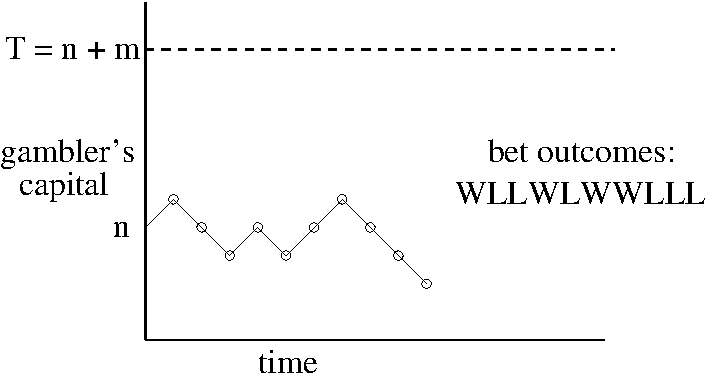
\includegraphics[height=2.5in]{figures/walk1}}
  \caption{\em This is a graph of the gambler's capital versus time
  for one possible sequence of bet outcomes.  At each time step, the
  graph goes up with probability $p$ and down with probability $1-p$.
  The gambler continues betting until the graph reaches either 0 or $T$.}
  \label{LN12:fig:walk1}
\end{figure}

In a \term{fair game}, the gambler is equally likely to win or lose
each bet, that is $p = 1/2$.  The corresponding random walk is called
\term{unbiased}.  The gambler is more likely to win if $p>1/2$ and
less likely to win if $p<1/2$; these random walks are called
\term{biased}.  We want to determine the probability that the walk
terminates at boundary $T$, namely, the probability that the gambler
is a winner.  We'll do this by showing that the probability satisfies
a simple linear recurrence and solving the recurrence, but before we
derive the probability, let's just look at what it turns out to be.

\begin{staffnotes}

\textcolor{blue}{Make this a pset problem}

\subsection{The Probability Space}

Each random-walk game corresponds to a path like the one in
Figure~\ref{LN12:fig:walk1} that starts at the point $(n,0)$.  A winning path
never touches the $x$ axis and ends when it first touches the line $y=T$.
Likewise, a losing path never touches the line $y=T$ and ends when it first
touches the $x$ axis.

\textcolor{red}{figure causing errors omitted here}
\iffalse

\setlength{\unitlength}{0.0125in}
%
\begingroup\makeatletter\ifx\SetFigFont\undefined
% extract first six characters in \fmtname
\def\x#1#2#3#4#5#6#7\relax{\def\x{#1#2#3#4#5#6}}%
\expandafter\x\fmtname xxxxxx\relax \def\y{splain}%
\ifx\x\y   % LaTeX or SliTeX?
\gdef\SetFigFont#1#2#3{%
  \ifnum #1<17\tiny\else \ifnum #1<20\small\else
  \ifnum #1<24\normalsize\else \ifnum #1<29\large\else
  \ifnum #1<34\Large\else \ifnum #1<41\LARGE\else
     \huge\fi\fi\fi\fi\fi\fi
  \csname #3\endcsname}%
\else
\gdef\SetFigFont#1#2#3{\begingroup
  \count@#1\relax \ifnum 25<\count@\count@25\fi
  \def\x{\endgroup\@setsize\SetFigFont{#2pt}}%
  \expandafter\x
    \csname \romannumeral\the\count@ pt\expandafter\endcsname
    \csname @\romannumeral\the\count@ pt\endcsname
  \csname #3\endcsname}%
\fi
\fi\endgroup
\begin{picture}(300,175)(0,-10)
\path(40,160)(40,0)
\path(20,40)(300,40)
\dottedline{5}(20,140)(300,140)
\path(40,80)(60,100)(80,80)
	(100,100)(120,120)(140,100)
	(160,120)(180,100)(200,80)
	(220,60)(240,80)(260,100)
	(280,120)(300,140)
\put(0,140){\makebox(0,0)[lb]{\smash{{{\SetFigFont{12}{14.4}{rm}T}}}}}
\put(0,40){\makebox(0,0)[lb]{\smash{{{\SetFigFont{12}{14.4}{rm}0}}}}}
\put(60,20){\makebox(0,0)[lb]{\smash{{{\SetFigFont{12}{14.4}{rm}1}}}}}
\put(80,20){\makebox(0,0)[lb]{\smash{{{\SetFigFont{12}{14.4}{rm}2}}}}}
\put(100,20){\makebox(0,0)[lb]{\smash{{{\SetFigFont{12}{14.4}{rm}3}}}}}
\put(0,80){\makebox(0,0)[lb]{\smash{{{\SetFigFont{12}{14.4}{rm}n}}}}}
\end{picture}
\fi

Any length $k$ path can be characterized by the history of wins and losses
on individual \$1 bets, so we use a length $k$ string of $W$'s and $L$'s to
model a path, and assign probability $p^rq^{k-r}$ to a string that contains
$r$ $W$'s.  The \emph{outcomes} in our sample space will be precisely those
string corresponding to winning or losing walks, that is, when $r=2k$.

What about the infinite walks in which the gambler plays forever, neither
reaching his target nor going bankrupt?  A recitation problem will show the
probability of playing forever is zero, so we don't need to include any
such outcomes in our sample space.

As a sanity check on this definition of the probability space, we should
verify that the sum of the outcome probabilities is one, but we omit this
calculation.

\iffalse
To do this, we let $X$ be any string of $W$'s and $L$'s, and let $[X]$ be
the event consisting of the outcomes that begin with $X$.  If $X$ itself
is not an outcome but begins with an outcome, then $[X] = \emptyset$ so
$\pr{[X]} = 0$.  On the other hand, if no prefix of $X$ is an outcome,
then it's easy to verify by induction on $k$ that $\pr{[X]} = p^rq^{k-r}$.
length $k$

\textcolor{blue}{COMPLETE}

We'll leave this to the reader.

\fi

\end{staffnotes}

%\subsection{The Probability of Winning}

%\subsubsection{The Unbiased Game}

Let's begin by supposing the coin is fair, the gambler starts with $100$
dollars, and he wants to double his money.  That is, he plays until he
goes broke or reaches a target of $200$ dollars.  Since he starts
equidistant from his target and bankruptcy, it's clear by symmetry that
his probability of winning in this case is 1/2.

We'll show below that starting with $n$ dollars and aiming for a target of
$T \geq n$ dollars, the probability the gambler reaches his target before
going broke is $n/T$.  For example, suppose he want to win the same \$100,
but instead starts out with \$500.  Now his chances are pretty good: the
probability of his making the 100 dollars is $5/6$.  And if he started
with one million dollars still aiming to win \$100 dollars he almost
certain to win: the probability is $1M/(1M + 100) > .9999$.

So in the fair game, the larger the initial stake relative to the target,
the higher the probability the gambler will win, which makes some
intuitive sense.  But note that although the gambler now wins nearly all
the time, the game is still fair.  When he wins, he only wins \$100; when
he loses, he loses big: \$1M.  So the gambler's average win is actually
zero dollars.

\begin{staffnotes}

\begin{example}
Suppose Albert starts with \$100, and Eric starts with \$10.  They flip a
fair coin, and every time a Head appears, Albert wins \$1 from Eric, and
vice versa for Tails.  They play this game until one person goes bankrupt.
What is the probability of Albert winning?

This problem is identical to the Gambler's Ruin problem with $n=100$ and
$T=100+10=110$.  The probability of Albert winning is $100/110 = 10/11$,
namely, the ratio of his wealth to the combined wealth.  Eric's chances of
winnning are $1/11$.
\end{example}
\end{staffnotes}

%\subsubsection{The Biased Game}

Now suppose instead that the gambler chooses to play roulette in an
American casino, always betting \$1 on red.  A roulette wheel has 18 black
numbers, 18 red numbers, and 2 green numbers, designed so that each number
is equally likely to appear.  So this game is slightly biased against the
gambler: the probability of winning a single bet is $p = 18/38 \approx
0.47$.  It's the two green numbers that slightly bias the bets and give
the casino an edge.  Still, the bets are almost fair, and you might expect
that starting with \$500, the gambler has a reasonable chance of winning
\$100 ---the 5/6 probability of winning in the unbiased game surely gets
reduced, but perhaps not too drastically.

Not so!  The gambler's odds of winning \$100 making one dollar bets
against the ``slightly'' unfair roulette wheel are less than 1 in 37,000.
If that seems surprising, listen to this: \emph{no matter how much money}
the gambler has to start ---\$5000, \$50,000, $\$5 \cdot 10^{12}$ ---his
odds are still less than 1 in 37,000 of winning a mere 100 dollars!

Moral:  Don't play!

The theory of random walks is filled with such fascinating and
counter-intuitive conclusions.

\subsection{A Recurrence for the Probability of Winning}

The probability the gambler wins is a function of his initial capital,
$n$, his target, $T \geq n$, and the probability, $p$, that he wins an
individual one dollar bet.  Let's let $p$ and $T$ be fixed, and let $w_n$
be the gambler's probabiliity of winning when his initial capital is $n$
dollars.  For example, $w_0$ is the probability that the gambler will win
given that he starts off broke and $w_T$ is the probability he will win if
he starts off with his target amount, so clearly
\begin{align}
w_0 & = 0,\label{LN12:w0}\\
w_T & = 1. \label{LN12:wT}
\end{align}

Otherwise, the gambler starts with $n$ dollars, where $0 < n < T$.
Consider the outcome of his first bet.  The gambler wins the first bet
with probability $p$.  In this case, he is left with $n+1$ dollars and
becomes a winner with probability $w_{n+1}$.  On the other hand, he loses
the first bet with probability $q \eqdef 1-p$.  Now he is left with $n-1$
dollars and becomes a winner with probability $w_{n-1}$.  By the Total
Probability Rule, he wins with probability $w_n = p w_{n+1} + q w_{n-1}$.
Solving for $w_{n+1}$ we have
\begin{equation}\label{LN12:rec1}
w_{n+1} = \frac{w_n}{p} -r w_{n-1}
\end{equation}
where
\[
r \eqdef \frac{q}{p}.
\]

This recurrence holds only for $n+1 \leq T$, but there's no harm in
using~\eqref{LN12:rec1} to define $w_{n+1}$ for all $n+1 >1$.  Now, letting
\[
W(x) \eqdef w_0 + w_1x + w_2x^2 + \cdots
\]
be the generating function for the $w_n$, we derive from~\eqref{LN12:rec1}
and~\eqref{LN12:w0} using our generating function methods that
\iffalse
\[
\frac{xW(x)}{p} - \frac{q}{p}x^2W(x) = W(x) - w_1x,
\]
so
\fi
\begin{equation}\label{LN12:Wx}
xW(x) = \frac{w_1x}{(1-x)(1-rx)},
\end{equation}
%= \frac{w_1x}{(q/p)x^2-(x/p)+1}

so if $p \neq q$, then using partial fractions we can calculate that

\begin{staffnotes}
\begin{equation}\label{LN12:WAB}
W(x)= \frac{A}{1-x} + \frac{B}{1-(q/p)x}.
\end{equation}
where $A=w_1/(1-(q/p))$

From~\eqref{LN12:Wx} and~\eqref{LN12:WAB}, we have
\[
w_1x = A(1-(q/p)x) + B(1-x).
\]
Letting $x=1$, we get $A=w_1/(1-(q/p))$, and letting $x=p/q$, we get
$B=-w_1/(1-(q/p))$, so

\end{staffnotes}

\[
W(x) = \frac{w_1}{r-1} \paren{\frac{1}{1-rx} - \frac{1}{1-x}},
\]
which implies
\begin{equation}\label{LN12:withw1}
w_n = w_1\frac{r^n - 1}{r-1}.
\end{equation}

Now we can use~\eqref{LN12:withw1} to solve for $w_1$ by letting $n=T$ to get
\begin{staffnotes}

\[
1=w_T = \frac{w_1}{(q/p)-1}\paren{\paren{\frac{q}{p}}^T - 1}
\]
so
\end{staffnotes}

\[
w_1= \frac{r - 1}{r^T-1}.
\]
Plugging this value of $w_1$ into~\eqref{LN12:withw1}, we finally arrive at
the solution:
\begin{equation}\label{LN12:wnsol}
w_n = \frac{r^n-1}{r^T -1}. 
\end{equation}

\iffalse
Our derivation of~(\ref{LN12:wnsol}) ensures that it gives a formula for $w_n$
which satisfies~(\ref{LN12:rec1}) and has the right values at $n=0$ and $n=T$.
Moreover, the values determined by~(\ref{LN12:wnsol}) are the \emph{only ones}
that satisfy~(\ref{LN12:rec1}) and the boundary conditions at $0$ and $T$,
though we won't prove this.  This implies that the Gambler's probability
of winning is indeed given by~(\ref{LN12:wnsol}).
\fi

The expression~\eqref{LN12:wnsol} for the probability that the Gambler wins
in the biased game is a little hard to interpret.  There is a simpler
upper bound which is nearly tight when the gambler's starting capital is
large and the game is biased {\em against} the
gambler.  Then both the numerator and denominator in the quotient
in~\eqref{LN12:wnsol} are positive, and the quotient is less than one.  This
implies that
\[
w_n < \frac{r^n}{r^T} = r^{T-n}, 
\]
which proves:
\begin{corollary}\label{LN12:biaswincor}
  In the Gambler's Ruin game with probability $p< 1/2$ of winning each
  individual bet, with initial capital, $n$, and target, $T$,
\begin{equation}\label{LN12:biaswinsimp}
\pr{\text{the gambler is a winner}} < \paren{\frac{p}{q}}^{T-n}
\end{equation}
\end{corollary}

The amount $T-n$ is called the Gambler's \emph{intended profit}.  So the
gambler gains his intended profit before going broke with probability at
most $p/q$ raised to the intended-profit power.  Notice that this upper
bound does not depend on the gambler's starting capital, but only on his
intended profit.  This has the amazing consequence we announced above:
\emph{no matter how much money he starts with}, if he
makes \$1 bets on red in roulette aiming to win \$100, the
probability that he wins is less than
\[
\paren{\frac{18/38}{20/38}}^{100} = \paren{\frac{9}{10}}^{100} < \frac{1}{37,648}.
\]

The bound~(\ref{LN12:biaswinsimp}) is exponential in the intended profit.  So,
for example, doubling his intended profit will square his probability of
winning.  In particular, the probability that the gambler's stake goes up
$200$ dollars before he goes broke playing roulette is at most
\[
(9/10)^{200} = ((9/10)^{100})^2 = \left(\frac{1}{37,648}\right)^2,
\]
which is about 1 in 70 billion.

\begin{staffnotes}

The odds of winning a little money are not so bad.
Applying the exact formula~\eqref{LN12:wnsol}, we find that the probability
of winning \$10 before losing \$10 is
\[
\frac{\paren{\frac{20/38}{18/38}}^{10} - 1}
              {\paren{\frac{20/38}{18/38}}^{20} - 1}
  = 0.2585\dots.
\]
This is somewhat worse than the 1 in 2 chance in the fair game, but not
dramatically so.

\end{staffnotes}

The solution~(\ref{LN12:wnsol}) only applies to biased walks, but the method
above works just as well in getting a formula for the unbiased case
(except that the partial fractions involve a repeated root).  But it's
simpler settle the fair case simply by taking the limit as $r$
approaches 1 of~\eqref{LN12:wnsol}.  By L'Hopital's Rule this limit is $n/T$,
as we claimed above.

\subsection{Intuition}

Why is the gambler so unlikely to make money when the game is slightly
biased against him?  Intuitively, there are two forces at work.  First,
the gambler's capital has random upward and downward {\em swings} due to
runs of good and bad luck.  Second, the gambler's capital will have a
steady, downward {\em drift}, because the negative bias means an average
loss of a few cents on each \$1 bet.  The situation is shown in
Figure~\ref{LN12:fig:walk2}.

\begin{staffnotes}

For example, in roulette the gambler wins a dollar with probability $9/19$
and loses a dollar with probability $10/19$.  Therefore, his average
return on each bet is $9/10 - 10/19 = - 1/19 \approx -0.053$ dollars.
That is, on each bet his capital is can be expected to drift downward by a
little over 5 cents.

\end{staffnotes}

Our intuition is that if the gambler starts with, say, a billion dollars,
then he is sure to play for a very long time, so at some point there
should be a lucky, upward swing that puts him \$100 ahead.  The problem is
that his capital is steadily drifting downward.  If the gambler does not
have a lucky, upward swing early on, then he is doomed.  After his capital
drifts downward a few hundred dollars, he needs a huge upward swing to
save himself.  And such a huge swing is extremely improbable.  As a rule
of thumb, \emph{drift dominates swings} in the long term.

%\begin{nooutline}
\begin{figure}
\centerline{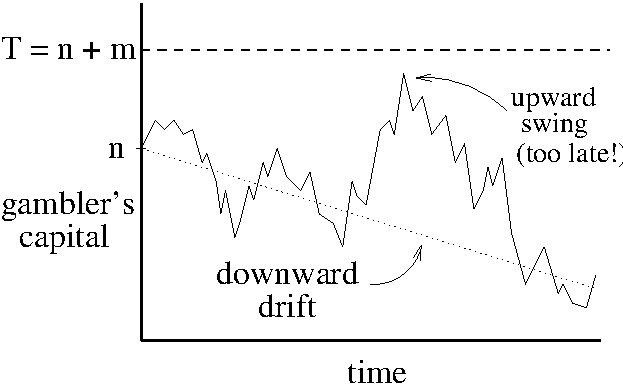
\includegraphics[height=2.5in]{figures/walk2}}
\caption{\em In an unfair game, the gambler's capital swings randomly up
and down, but steadily drifts downward.  If the gambler does not have
a winning swing early on, then his capital drifts downward, and later
upward swings are insufficient to make him a winner.}
\label{LN12:fig:walk2}
\end{figure}
%\end{nooutline}

\begin{staffnotes}

We can quantify these drifts and swings.  After $k$ rounds for $k \le
\min(m,n)$, the number of wins by our player has a binomial distribution
with parameters $p < 1/2$ and $k$.  His expected win on any single bet is
$p-q = 2p-1$ dollars, so his expected capital is $n-k(1-2p)$.  Now to be a
winner, his actual number of wins must exceed the expected number by
$m+k(1-2p)$.  But we saw before that the binomial distribution has a
standard deviation of only $\sqrt{kp(1-p)}$.  So for the gambler to win,
he needs his number of wins to deviate by
\[
\frac{m+k(1-2p)}{\sqrt{kp(1-2p)}}=\Theta(\sqrt{k})
\]
times its standard deviation.  In our study of binomial tails we saw that
this was extremely unlikely.

In a fair game, there is no drift; swings are the only effect.  In the
absence of downward drift, our earlier intuition is correct.  If the
gambler starts with a trillion dollars then almost certainly there
will eventually be a lucky swing that puts him \$100 ahead.

If we start with \$10 and play to win only \$10 more, then the difference
between the fair and unfair games is relatively small. We saw that the
probability of winning is $1/2$ versus about $1/4$.  Since swings of \$10
are relatively common, the game usually ends before the gambler's capital
can drift very far.  That is, the game does not last long enough for drift
to dominate the swings.

\subsection{How Long a Walk?}

Now that we know the probability, $w_n$, that the gambler is a winner in
both fair and unfair games, we consider how many bets he needs on average
to either win or go broke.

\subsection{Duration of a Biased Walk}

Let $Q$ be the number of bets the gambler makes until the game ends.  Since
the gambler's expected win on any bet is $2p-1$, Wald's Theorem should tell
us that his game winnings, $G$, will have expectation $\expect{Q}(2p-1)$.
That is,nn
\begin{equation}\label{LN12:gw}
\expect{G} = (2p-1)\expect{Q},
\end{equation}

In an unbiased game~(\ref{LN12:gw}) is trivially true because both $2p-1$ and
the expected overall winnings, $\expect{G}$, are zero.  On the other hand,
in the unfair case, $2p-1 \neq 0$.  Also, we know that
\[
\expect{G} = w_n(T-n) - (1-w_n)n = w_nT-n.
\]
So assuming~(\ref{LN12:gw}), we conclude
\begin{theorem}\label{LN12:ExQthm}
In the biased Gambler's Ruin game with initial capital, $n$, target,
$T$, and probability, $p \neq 1/2$, of winning each bet,
\begin{equation}\label{LN12:ExQ}
\expect{\text{number of bets till game ends}} =
\frac{\pr{\text{gambler is a winner}}T-n}{2p-1}.
\end{equation}
\end{theorem}

The only problem is that~(\ref{LN12:gw}) is not a special case of Wald's
Theorem because $G = \sum_{i=1}^Q G_i$ is not a sum of \emph{nonnegative}
variables: when the gambler loses the $i$th bet, the random variable $G_i$
equals $-1$.  However, this is easily dealt with.\footnote{The random variable
$G_i+1$ is nonnegative, and $\expcond{G_i+1}{Q \geq i} =
\expcond{G_i}{Q\geq i}+1 = 2p$, so by Wald's Theorem
\begin{equation}\label{LN12:G1}
\expect{\sum_{i=1}^Q (G_i+1)}  = 2p\expect{Q}.
\end{equation}
But
\begin{eqnarray}q1
\expect{\sum_{i=1}^Q (G_i+1)} & = & \expect{\sum_{i=1}^Q G_i + \sum_{i=1}^Q 1}\notag\\
   & = & \expect{(\sum_{i=1}^Q G_i) + Q}\notag\\
   & = & \expect{\sum_{i=1}^Q G_i} + \expect{Q}\notag\\
   & = & \expect{G} + \expect{Q}\label{LN12:GQ}.
\end{eqnarray}
Now combining~(\ref{LN12:G1}) and~(\ref{LN12:GQ}) confirms the truth of our
assumption~(\ref{LN12:gw}).}

\begin{example}
If the gambler aims to profit \$100 playing roulette with $n$ dollars to
start, he can expect to make $((n+100)/37,648 - n)/(2(18/38) - 1) \approx
19n$ bets before the game ends.  So he can enjoy playing for a good while
before almost surely going broke.
\end{example}


\subsection{Duration of an Unbiased Walk}

This time, we need the more general approach of recurrences to handle the
unbiased case.  We consider the expected number of bets as a
function of the gambler's initial capital.  That is, for fixed $p$ and $T$,
let $e_n$ be the expected number of bets until the game ends when the
gambler's initial capital is $n$ dollars.  Since the game is over in no
steps if $n=0$ or $T$, the boundary conditions this time are $e_0=e_T=0$.

Otherwise, the gambler starts with $n$ dollars, where $0 < n < T$.
Now by the conditional expectation rule, the expected number of steps can
be broken down into the expected number of steps given the outcome of the
first bet weighted by the probability of that outcome.  That is,
\[
e_n = p\expcond{Q}{\text{gambler wins first bet}} +
q\expcond{Q}{\text{gambler loses first bet}}.
\]
But after the gambler wins the first bet, his capital is $n+1$, so
he can expect to make another $e_{n+1}$ bets.  That is,
\[
\expcond{Q}{\text{gambler wins first bet}} = 1 + e_{n+1},
\]
and similarly, 
\[
\expcond{Q}{\text{gambler loses first bet}} = 1 + e_{n-1}.
\]
So we have
\[
e_n =  p(1 + e_{n+1}) +  q(1 + e_{n-1}) =  pe_{n+1} + qe_{n-1} + 1, 
\]
which yields the linear recurrence
\[
e_{n+1} = \frac{e_n}{p} - \frac{q}{p} e_{n-1} - \frac{1}{p}.
\]
For $p = q = 1/2$, this equation simplifies to
\begin{equation}\label{LN12:en2}
e_{n+1} = 2e_n - e_{n-1} - 2.
\end{equation}
There is a general theory for solving linear recurrences like~(\ref{LN12:en2})
in which the value at $n+1$ is a linear combination of values at some
arguments $k<n+1$ plus another simple term---in this case plus the constant
$-2$.  This theory implies that
\begin{equation}\label{LN12:Tn}
e_n  = (T - n)n.
\end{equation}
Fortunately, we don't need the general theory to \emph{verify} this
solution.  Equation~(\ref{LN12:Tn}) can be verified routinely from the boundary
conditions and~(\ref{LN12:en2}) using strong induction on $n$.

So we have shown
\begin{theorem}\label{LN12:fairtime}
In the unbiased Gambler's Ruin game with initial capital, $n$, and target,
$T$, and probability, $p = 1/2$, of winning each bet,
\begin{equation}
\expect{\text{number of bets till game ends}} = n(T-n).
\end{equation}
\end{theorem}

Another way to phrase Theorem~\ref{LN12:fairtime} is
\begin{equation}\label{LN12:mn}
\expect{\text{number of bets till game ends}} = \text{initial capital}
\cdot \text{intended profit}.
\end{equation}

Now for example, we can conclude that if the gambler starts with \$10
dollars and plays until he is broke or ahead \$10, then $10 \cdot 10 = 100$
bets are required on average.  If he starts with \$500 and plays until he
is broke or ahead \$100, then the expected number of bets until the game is
over is $500 \times 100 = 50,000$.

Notice that~(\ref{LN12:mn}) is a very simple answer that cries out for an
intuitive proof, but we have not found one.

\end{staffnotes}

\iffalse

\textcolor{blue}{Below is my try at the suggestion of Santosh and Adam
  Kalai for an example requiring a Pairwise \emph{Uncorrellated}
  Sampling Theorem.  But I don''t think this goes anywhere.}

\subsection{Fluctuations in an Unbiased Walk}

Let's consider the probability that the game ends within $k$ flips.  This
number is awkward to calculate explicitly, but we will be able to estimate
it using our methods for estimating expected deviation from the mean.

Let $C_k$ be the gamblers capital after $k$ flips.  That is,
\[
C_k \eqdef n + \sum_{i=1}^k G_i.
\]
In the unbiased case, the expected win on one flip is zero, so since $C_k$
is the sum of variables which have expectation 0, it follows that
$\expect{C_k} = 0$.  What about $\variance{C_k}$?  We will prove that
\begin{equation}\label{LN12:sumvarg}
\variance{C_k} = \sum_{i=1}^k \variance{G_i}.
\end{equation}

Note that for $i \neq j$, $G_i$ and $G_j$ are not independent, and so we
cannot appeal to pairwise independent additivity of variance to
prove~(\ref{LN12:sumvarg}).  For example, if $G_i = 0$, then the game has
stopped before the $i$th flip, so if $j > i$, then $G_j = 0$.  On the
other hand, the probability that $G_j = 0$ is less than one, because there
is some positive probability that the game will continue for more than $j$
flips (except for the degenerate case when $n=1 and T=2$).  That is,
\[
\prcond{G_j = 0}{G_i = 0} = 1 > \pr{G_j = 0},
\]
confirming nonindependence.

However, inspection of the proof of pairwise independent additivity of
variance shows that it didn't really require pairwise independence!  The
only property of the variables being added is that they be pairwise
\emph{uncorrelated}:

\begin{definition*}
Random variables $R$ and $S$ are \emph{uncorrelated} iff
\begin{equation}\label{LN12:uncor}
\expect{RS} = \expect{R}\expect{S}.
\end{equation}
\end{definition*}

\begin{lemma}\label{LN12:Guncor}
For $i \neq j$, $G_i$ and $G_j$ are uncorrelated.
\end{lemma}
\fi

\begin{staffnotes}

\subsection{Quit While You Are Ahead}

Suppose that the gambler never quits while he is ahead.  That is, he
starts with $n>0$ dollars, ignores any target $T$, but plays until he is
flat broke.  Then it turns out that if the game is not favorable, \ie $p
\leq 1/2$, the gambler is sure to go broke.  In particular, he is even
sure to go broke in a ``fair'' game with $p = 1/2$.

If the game is favorable to the gambler, \ie $p>1/2$, then there is a
positive probability that the gambler will play forever.  We'll leave a
proof of this to Problem\ref{}.

\begin{lemma}\label{LN12:go broke}
If the gambler starts with one or more dollars and plays a fair game until
he is broke, then he will go broke with probability 1.
\end{lemma}

\begin{proof}
If the gambler has initial capital $n$ and goes broke in a game without
reaching a target $T$, then he would also go broke if he were playing and
ignored the target.  So the probability that he will lose if he keeps
playing without stopping at any target $T$ must be at least as large as the
probability that he loses when he has a target $T>n$.

But we know that in a fair game, the probability that he loses is $1 -
n/T$.  This number can be made arbitrarily close to 1 by choosing a
sufficiently large value of $T$.  Hence, the probability of his losing
while playing without any target has a lower bound arbitrarily close to 1,
which means it must in fact be 1.
\end{proof}

So even if the gambler starts with a million dollars and plays a perfectly
fair game, he will eventually lose it all with probability 1.  In fact, if
the game is unfavorable, then Theorem~\ref{LN12:ExQthm} and
Corollary~\ref{LN12:biaswincor} imply that his expected time to go broke is
essentially proportional to his initial capital, \ie $\Theta(n)$.

But there is good news: if the game is fair, he can ``expect'' to play for
a very long time before going broke; in fact, he can expect to play
forever!

\begin{lemma}\label{LN12:play forever}
If the gambler starts with one or more dollars and plays a fair game until
he goes broke, then his expected number of plays is infinite.
\end{lemma}

\begin{proof}
Consider the gambler's ruin game where the gambler starts with initial
capital $n$, and let $u_n$ be the expected number of bets for
the \emph{unbounded} game to end.  Also, choose any $T \geq n$, and as
above, let $e_n$ be the expected number of bets for the game to end when
the gambler's target is $T$.

The unbounded game will have a larger expected number of bets compared to
the bounded game because, in addition to the possibility that the gambler
goes broke, in the bounded game there is also the possibility that the
game will end when the gambler reaches his target, $T$.  That is,
\[
u_n \geq e_n.
\]
So by~(\ref{LN12:Tn}), 
\[
u_n \geq n(T-n).
\]
But $n \geq 1$, and $T$ can be any number greater than or equal to $n$, so
this lower bound on $u_n$ can be arbitrarily large.  This implies that
$u_n$ must be infinite.

Now by Lemma~\ref{LN12:go broke}, with probability 1, the unbounded game ends
when the gambler goes broke.  So the expected time for the unbounded game
to \emph{end} is the \emph{same} as the expected time for the gambler to
\emph{go broke}.  Therefore, the expected time to go broke is infinite.
\end{proof}

In particular, even if the gambler starts with just one dollar, his
expected number of plays before going broke is infinite!  Of course, this
does not mean that it is likely he will play for long.  For example, there
is a 50\% chance he will lose the very first bet and go broke right away.

Lemma~\ref{LN12:play forever} says that the gambler can ``expect'' to play
forever, while Lemma~\ref{LN12:go broke} says that with probability 1 he will
go broke.  These Lemmas sound contradictory, but our analysis showed that
they are not.  A moral is that naive intuition about ``expectation'' is
misleading when we consider limiting behavior according to the technical
mathematical definition of expectation.

\end{staffnotes}

%% Gamblers' Ruin Problems %%%%%%%%%%%%%%%%%%%%%%%%%%%%%%%%%%%%%%%%%%%%%%%%%%%%

\begin{problems}
\classproblems
\pinput{CP_gambler_ruin_recurrences}

\homeworkproblems
\pinput{PS_drunken_sailor}
\end{problems}


%% Random Walks on Graphs %%%%%%%%%%%%%%%%%%%%%%%%%%%%%%%%%%%%%%%%%%%%%%%%%%%%%
\section{Random Walks on Graphs}\label{Google_sec}

\begin{staffnotes}

\hyperdef{page}{rank}{Random walks on graphs arise in all sorts of
  applications.  One interesting example is Google and page rank, which
  we'll explore in this section.}

\end{staffnotes}

The hyperlink structure of the World Wide Web can be described as a
digraph.  The vertices are the web pages with a directed edge from vertex
$x$ to vertex $y$ if $x$ has a link to $y$.  For example, in the following
graph the vertices $x_1, \ldots, x_n$ correspond to web pages and
$\diredge{x_i}{x_j}$ is a directed edge when page $x_i$ contains a
hyperlink to page $x_j$.

\mfigure{!}{2in}{figures/randomWalkFigs/webGraph}

The web graph is an enormous graph with many billions and probably even
trillions of vertices.  At first glance, this graph wouldn't seem to be very
interesting.  But in 1995, two students at Stanford, \index{Page, Larry}
Larry Page and index{Brin, Sergey} Sergey Brin realized that the structure
of this graph could be very useful in building a search engine.
Traditional document searching programs had been around for a long time
and they worked in a fairly straightforward way.  Basically, you would
enter some search terms and the searching program would return all
documents containing those terms.  A relevance score might also be
returned for each document based on the frequency or position that the
search terms appeared in the document.  For example, if the search term
appeared in the title or appeared $100$ times in a document, that document
would get a higher score.  So if an author wanted a document to get a
higher score for certain keywords, he would put the keywords in the title
and make it appear in lots of places.  You can even see this today with
some bogus web sites.

This approach works fine if you only have a few documents that match a
search term.  But on the web, there are billions of documents and millions
of matches to a typical search.

For example, a few years ago a search on Google for ``math for computer
science notes'' gave 378,000 hits!  How does Google decide which 10 or 20
to show first?  It wouldn't be smart to pick a page that gets a high
keyword score because it has ``math math $\dots$ math'' across the front
of the document.

One way to get placed high on the list is to pay Google an advertising
fees ---and Google gets an enormous revenue stream from these fees.  Of
course an early listing is worth a fee only if an advertiser's target
audience is attracted to the listing.  But an audience does get attracted
to Google listings because its ranking method is really good at
determining the most relevant web pages.  For example, Google demonstrated
its accuracy in our case by giving first rank to the Fall 2002 open
courseware page for 6.042 \texttt{:-)} .  So how did Google know to pick
6.042 to be first out of $378,000$?

Well back in 1995, Larry and Sergey got the idea to allow the digraph
structure of the web to determine which pages are likely to be the most
important.

\subsection{A First Crack at Page Rank}

Looking at the web graph, any idea which vertex/page might be the best to
rank $1$st?  Assume that all the pages match the search terms for now.
Well, intuitively, we should choose $x_2$, since lots of other pages point
to it.  This leads us to their first idea: try defining the \term{page
  rank} of $x$ to be the number of links pointing to $x$, that is,
$\text{indegree}(x)$.  The idea is to think of web pages as voting for the
most important page ---the more votes, the better rank.

Of course, there are some problems with this idea.  Suppose you wanted
to have your page get a high ranking.  One thing you could do is to
create lots of dummy pages with links to your page.

\mfigure{!}{1.5in}{figures/randomWalkFigs/dummy}

There is another problem ---a page could become unfairly influential by
having lots of links to other pages it wanted to hype.

\mfigure{!}{1.5in}{figures/randomWalkFigs/outDegree}

So this strategy for high ranking would amount to, ``vote early, vote
often,'' which is no good if you want to build a search engine that's
worth paying fees for.  So, admittedly, their original idea was not so
great.  It was better than nothing, but certainly not worth billions of
dollars.

\subsection{Random Walk on the Web Graph}

But then Sergey and Larry thought some more and came up with a couple of
improvements.  Instead of just counting the indegree of a vertex, they
considered the probability of being at each page after a long random walk
on the web graph.  In particular, they decided to model a user's web
experience as following each link on a page with uniform probability.
That is, they assigned each edge $x \rightarrow y$ of the web graph with a
probability conditioned on being on page $x$:
\[
\prcond{\text{follow link}\ \diredge{x}{y}}{ \text{at page $x$}} \eqdef
\frac{1}{\text{outdegree}(x)}.
\]
The user experience is then just a \idx{random walk} on the web graph.

For example, if the user is at page $x$, and there are three links from
page $x$, then each link is followed with probability $1/3$.

We can also compute the probability of arriving at a particular page, $y$,
by summing over all edges pointing to $y$.  We thus have
\begin{eqnarray}
  \pr{\text{go to $y$}} &=&  \sum_{\text{edges}\ \diredge{x}{y}}
  \prcond{\text{follow link}\ \diredge{x}{y}}{\text{at page $x$}} \cdot
  \pr{\text{at page $x$}} \nonumber\\
  &=& \sum_{\text{edges}\ \diredge{x}{y}} \frac{\pr{\text{at
      $x$}}}{\text{outdegree}(x)} \label{LN12:stepprob}
\end{eqnarray}
For example, in our web graph, we have
\[ \pr{\text{go to $x_4$}} = \frac{\pr{\text{at $x_7$}}}{2} +
\frac{\pr{\text{at $x_2$}}}{1} \ .
\]
One can think of this equation as $x_7$ sending half its probability to
$x_2$ and the other half to $x_4$. The page $x_2$ sends all of its
probability to $x_4$.

There's one aspect of the web graph described thus far that doesn't mesh
with the user experience ---some pages have no hyperlinks out.  Under the
current model, the user cannot escape these pages.  In reality, however,
the user doesn't fall off the end of the web into a void of nothingness.
Instead, he restarts his web journey.

To model this aspect of the web, Sergey and Larry added a supervertex to the
web graph and had every page with no hyperlinks point to it.  Moreover,
the supervertex points to every other vertex in the graph, allowing you to
restart the walk from a random place.  For example, below left is a graph
and below right is the same graph after adding the supervertex $x_{N+1}$.

\bigskip\centerline{
  \resizebox{!}{1.3in}{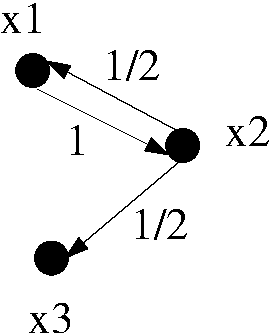
\includegraphics{figures/randomWalkFigs/adjMatrix2}}
  \hspace{2cm}
  \resizebox{!}{1.5in}{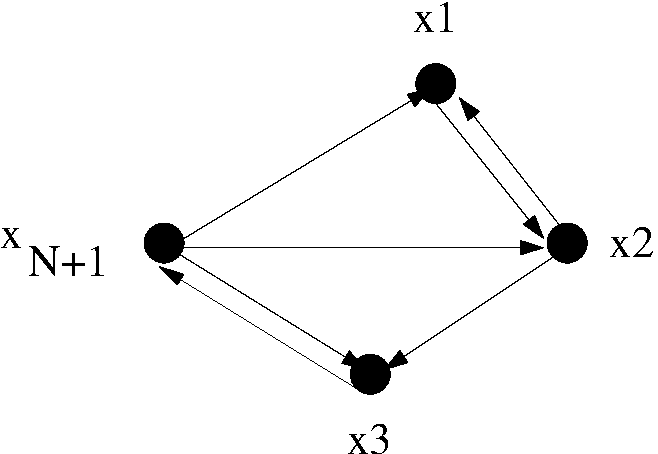
\includegraphics{figures/randomWalkFigs/sinkGraph}}
}\bigskip

The addition of the supervertex also removes the possibility that the value
$1/\text{outdegree}(x)$ might involve a division by zero.

\subsection{Stationary Distribution \& Page Rank}

The basic idea of \idx{page rank} is just a stationary distribution over
the web graph,
\begin{staffnotes}
(there are some more details, but this is the main idea)
\end{staffnotes}
so let's define a stationary distribution.

Suppose each vertex is assigned a probability that corresponds, intuitively,
to the likelihood that a random walker is at that vertex at a randomly
chosen time.  We assume that the walk never leaves the vertices in the graph,
so we require that
\begin{equation}\label{LN12:sum1}
\sum_{\text{vertices}\ x} \pr{\text{at $x$}} = 1.
\end{equation}

\begin{definition} An assignment of probabililties to vertices in a digraph
  is a \term{stationary distribution} if for all vertices $x$
\[
\pr{\text{at $x$}} = \pr{\text{go to $x$ at next step}}
\]
\end{definition}  

Sergey and Larry defined their page ranks to be a stationary distribution.
They did this by solving the following system of linear equations: find a
nonnegative number, $\text{PR}(x)$, for each vertex, $x$, such that

\begin{equation}\label{LN12:PReqs}
\text{PR}(x) = \sum_{\text{edges}\ \diredge{y}{x}} \frac{\text{PR}(y)}{\text{outdegree}(y)},
\end{equation}
corresponding to the intuitive equations given in \eqref{LN12:stepprob}.
These numbers must also satisfy the additional constraint corresponding
to~\eqref{LN12:sum1}:

\begin{equation}\label{LN12:sum1PR}
\sum_{\text{vertices}\ x} \text{PR}(x) = 1.
\end{equation}

So if there are $n$ vertices, then equations~\eqref{LN12:PReqs}
and~\eqref{LN12:sum1PR} provide a system of $n+1$ linear equations in the
$n$ variables, $\text{PR}(x)$.  Note that constraint~\eqref{LN12:sum1PR}
is needed because the remaining constraints~\eqref{LN12:PReqs} could be
satisfied by letting $\text{PR}(x)\eqdef 0$ for all $x$, which is useless.

Sergey and Larry were smart fellows, and they set up their page rank
algorithm so it would always have a meaningful solution.  Their addition
of a supervertex ensures there is always a \emph{unique} stationary
distribution.  Moreover, starting from \emph{any} vertex and taking a
sufficiently long random walk on the graph, the probability of being at
each page will get closer and closer to the stationary distribution.  Note
that general digraphs without supervertices may have neither of these
properties: there may not be a unique stationary distribution, and even
when there is, there may be starting points from which the probabilities
of positions during a random walk do not converge to the stationary
distribution.  

\begin{staffnotes}
Here's a note on solving the system of linear constraints, for the
interested reader.

Let $W$ be the $n \times n$ with the entry $w_{ij}$ (in row $i$ and
column $j$) having the value $w_{ij} = 1/\text{outdegree}(x_i)$ if edge
$x_i \rightarrow x_j$ exists, and $w_{ij} = 0$ otherwise.  For example, in
our last example with the 4-vertex graph (including the supervertex), we have
$W$ given by:
\[
\left( \begin{array}{cccc}
    0 & 1 & 0 & 0 \\
    \frac{1}{2} & 0 & \frac{1}{2} & 0 \\
    0 & 0 & 0 & 1\\
    \frac{1}{3} & \frac{1}{3} & \frac{1}{3} & 0 \end{array} \right)
\]

The system of linear equations can now be described by a single matrix
vector product equation $W^T \vec{P} = \vec{P}$, where $W^T$ denotes the
transpose of $W$, and $\vec{P}$ is the column vector of page probabilities
(ranks):
\[\vec{P}\eqdef
\left( \begin{array}{c}
    \text{PR}(x_1) \\
    \text{PR}(x_2) \\
    \vdots \\
    \text{PR}(x_n) \end{array} \right)
\]
So the $j$th entry of the solultion vector, $\vec{P}$, is
\[
\sum_{1\leq i \leq n} w_{ij} \cdot \text{PR}(x_i) =
\sum_{i \mid x_i \rightarrow x_j} \frac{\text{PR}(x_i)}{\text{outdegree}(x_i)},
\]
which is exactly the constraint corresponding to vertex $x_j$
in~\eqref{LN12:PReqs}.

If you have taken a linear algebra or numerical analysis course, you
realize that the vector of page ranks is just the \emph{principle
  eigenvector} of the matrix, $W$, of the web graph!  Once you've had such
a course, these values are easy to compute.  Of course, when you are
dealing with matrices of this size, the problem gets a little more
interesting.

\end{staffnotes}

Now just keeping track of the digraph whose vertices are billions of web
pages is a daunting task.  That's why Google is building power plants.
Indeed, Larry and Sergey named their system Google after the number
$10^{100}$ ---which called a ``googol'' ---to reflect the fact that the
web graph is so enormous.

Anyway, now you can see how 6.042 ranked first out of 378,000 matches.
Lots of other universities used our notes and presumably have links to the
6.042 open courseware site, and the university sites themselves are
legitimate, which ultimately leads to 6.042 getting a high page rank in
the web graph.

%% Random Walks on Graphs Problems %%%%%%%%%%%%%%%%%%%%%%%%%%%%%%%%%%%%%%%%%%%%
\begin{problems}

\classproblems
\pinput{CP_random_walk_stationary_distributions}
\pinput{CP_simple_google_graph}

\homeworkproblems
\pinput{PS_random_walk_strongly_connected}

\examproblems
\pinput{FP_uniform_stationary_distribution}

\end{problems}


%% Conclusion %%%%%%%%%%%%%%%%%%%%%%%%%%%%%%%%%%%%%%%%%%%%%%%%%%%%%%%%%%%%%%%%%
%\TBA{Conclusion...}

\endinput
